Все современные дифференциальные алгоритмы слежения за особенностями опираются на работу 1981 году Лукаса и Канаде \cite{lyka_kan}. В 1991 году математическая формулировка этого алгоритма была изменена, и стала основой для всех последующих обобщений с учетом аффинных искажений окрестности и освещенности. Путем замены соответствующих переменных на константы любой из них превращается в обычный алгоритм Lucas–Kanade.

\begin{enumerate}
\item Lucas–Kanade – особенность считается только смещающейся, без искажений;
\item Tomasi–Kanade – переформулирование Lucas–Kanade \cite{tom_lyk}. Движение считается смещением, и рассчитывается путем итеративного решения построенной системы линейных уравнений;
\item Shi–Tomasi–Kanade – учитывает аффинные искажения особенности \cite{shi_tom_lyk}.
%\item Jin–Favaro–Soatto – модификация Shi–Tomasi–Kanade с учетом аффинных изменений освещенности особенности
\end{enumerate}

\subsection{Lucas–Kanade}

Этот алгоритм в принципе применим для функций любой размерности $n$. Пусть $x$ – особенность первой функции $F$, необходимо найти такую точку $x+h$ функции $G$, что разность окрестностей этих точек по мере – минимальна.

Расстояние между окрестностями записывается в виде:

\numberwithin{equation}{section}
\begin{equation}
E=\sum [F(x+h)-G(x)]^2
\end{equation}

где $F(x)$, $G(x)$ - две функции.

Функцию $F(x)$ с помощью разложения в ряд Тейлора можно приближенно представить в виде:

\numberwithin{equation}{section}
\begin{equation}
F(x+h)\approx F(x)+h\frac{\partial}{\partial x}F(x)
\end{equation}

Используя это приближение, ищется минимум $E$ путем дифференцирования и приравнивания производной к нулю:

\[0=\frac{\partial}{\partial h} E\]
\[0 \approx \frac{\partial}{\partial h} \sum_x[F(x)+h\frac{\partial}{\partial h}-G(x)]^2\]
\[0 =\sum_x 2\frac{\partial F}{\partial x} [F(x)+h\frac{\partial F}{\partial x}-G(x)]^2\]

Отсюда смещение $h$ можно получить как:

\[h = \left[\sum(\frac{\partial F}{\partial x})^T[G(x)-T(x)]\right] \left[\sum(\frac{\partial F}{\partial x})^T(\frac{\partial F}{\partial x})^{-1}\right]\]

Как было указано ранее, задача слежения за особенностями без учета аффинных искажений является поиском величины оптического потока в наборе точек Поэтому метод Lucas-Kanade часто применяется для поиска оптического потока во всем изображении.

\subsection{Tomasi-Kanade}
В этом алгоритме движение особых точек также описывается смещением вида:
\[delta(x) = x + d.\]
Как и в предыдущем алгоритме, задача заключается в поиске такого $d$, при котором минимизируется разность окон особенностей:
\numberwithin{equation}{section}
\begin{equation}
\varepsilon =\sum_W \left[l(x+d,t+\tau)-l(x,t) \right]^2
\end{equation}
Опять же аналогично функция изображения раскладывается с помощью ряда Тейлора:
\numberwithin{equation}{section}
\begin{equation}
l(x+d,t+\tau) \approx l(x,t) + \nabla l(x,t)^\tau d+l_t(x,t)\tau
\end{equation}
Тогда разницу между окнами по мере можно переписать в виде:
\numberwithin{equation}{section}
\begin{equation}
\varepsilon =\sum_W \left( \nabla l(x,t)^\tau d+l_t(x,t)\tau \right)^2
\end{equation}
Дифференцировав это выражение по $d$ и приравняв производную к нулю, получаем линейную систему относительно $d$
$$Cd=g$$
где,$$C = \sum_W \begin{bmatrix}
I_u^2 & I_uI_v\\
I_ul_v & I_u^2
\end{bmatrix}$$

$$g=\tau\sum_W l_t \left | I_uI_v \right |^T$$
Из этой системы $d$ получается как:
$$d_k=C^{-1}g$$

С учетом приближения функции изображения с помощью ряда Тейлора, решение получается неточным. Для его уточнения удобно применить итеративную процедуру Ньютона-Рафсона. Т.е. полученное на первом шаге решение берется за новое первое приближение, уравнение снова и снова.

На каждом шаге рекомендуется пересчитывать окрестность особенности с помощью интерполирования для достижения субпиксельной точности нахождения положения особенности в новом кадре.

Если интервал времени между кадрами принять за 1, получается следующий алгоритм:
\[
\begin{cases}
$d_0 = 0$ \\
$d_{k+1}=d_k + C^{-1} \sum_W \left[ (I(x,t) - I(x+d_k,t + 1)) \nabla I (x,t) \right]$
\end{cases}
\]

Таким образом, этот алгоритм слежения фактически является поиском точки, в которой достигается минимум некоторой функции, методом градиентного спуска. Во время каждой итерации мы сдвигаемся вдоль направления градиента изображения в текущей точке.

\subsection{Shi-Tomasi-Kanade tracker}

В этом алгоритме впервые учитываются аффинные искажения изображения окрестности особых точек, поэтому движение пикселей окна особенности описывается в виде $Ax + d$, где $A$ - матрица $(2 \cdot 2)$, $а d$ - смещение $(2 \cdot 1)$.

Задача слежения за особенностью сводится к проблеме проблема определения параметров движения и искажения окна особенности, при которой минимизируется разность:
$$r=\iint_W [J(\Delta x+d)-I(x)]^2$$
где $W$ - окно особенности, а $w$ - весовая функция (может использовать, а может и быть равна 1 во всем окне), $J(x)$ и $I(x)$ - два изображения.

Выражение дифференцируется относительно параметров движения, и производная приравнивается к 0. Затем система линеаризуется с помощью разложения функции изображения в ряд Тейлора:
$$J(\Delta x+d)= J(x)+g^T(u)$$

Это дает нам линейную $6 \cdot 6$ систему:
$$Tz=a$$
, где в векторе $z$ объединены все искомые параметры:

$$z^T=\begin{bmatrix}
 d_{xx} & d_{yx} & d_{xy} & d_{yy} & d_x & d_y
\end{bmatrix}$$
Вектор ошибки a записывается в виде:
$$a=\iint_W [I(x)-J(x)]\begin{bmatrix}
xg_x\\
xg_y\\
yg_x\\
yg_y\\
g_x\\
g_y
\end{bmatrix}\omega dx$$
А матрицу размерности $6 \cdot 6$ $T$ можно представить следующим образом:
$$T=\iint_W [I(x)-J(x)]\begin{bmatrix}
U & V\\
V^T & Z
\end{bmatrix}\omega dx$$

$$U=\begin{bmatrix}
x^3g^3_x & x^3g_xg_y & xyg^3_x_x & xyg_xg_y \\
x^3g_xg_y & x^3g^3_y & xyg_xg_y & xyg^3_x \\
xyg^3_x & xyg_xg_y & y^3g^3_x & y^3g_xg_y \\
xyg_xg_y & xyg^3_y & y^3g_xg_y & y^3g^3_y
\end{bmatrix}$$

$$V^T=\begin{bmatrix}
xg^3_x & xg_xg_y & yg^3_x & yg_xg_y \\
xg_xg_y & xg^3_y & yg_xg_y & yg^3_y
\end{bmatrix}$$

$$Z=\begin{bmatrix}
g^3_x & g_xg_y \\
g_xg_y & g^3_y
\end{bmatrix}$$

Полученная система решается также итеративно по методу Ньютона-Рафсона.

Если движение считается не аффинным, а просто смещением, то первые четыре элемента искомого вектора $z$ обращаются в 0, и значимыми остаются только последние два. Алгоритм превращается в алгоритм Tomasi-Kanade.

\subsection{Иерархический метод}
Пирамидальный (иерархический) алгоритм Лукаса - Канаде в значительной степени использует классический метод. В методе используется пирамида изображений т.е. последовательность изображений, в которой каждое последующее получается из предыдущего уменьшением его размеров в два раза.

Каждое изображение последовательности, за исключением первого, получается как свертка предыдущего изображения со следующим фильтром:
(рис. \ref{pic:pyramid}).
Пирамидальный алгоритм Лукаса - Канаде для поиска потока в точке $(x_0,y_0)$.
\begin{enumerate}
\item По каждому из двух данных изображениям строится пирамида изображений
\item Для $i$ – го изображения пирамиды по первому и второму изображениям применяется классический KLT метод, с вектором начального приближения $2 \cdot d_{i+1}$, где $d_{i+1}$ – вектор потока, полученный на предыдущем уровне пирамиды.
\end{enumerate}
Для самого первого уровня этот вектор принимается равным (0,0).


\begin{figure}[ht]
\center{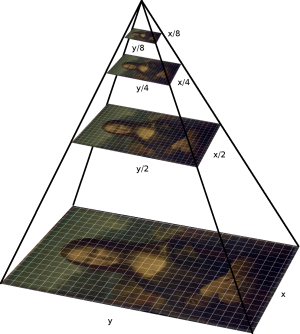
\includegraphics[width=0.6\linewidth]{pyramid}}
\caption{Пример пирамиды Гаусса}
\label{pic:pyramid}
\end{figure}